\documentclass{beamer}
\usepackage[spanish]{babel}
\usepackage[utf8]{inputenc}
\usepackage{graphicx} % Para insertar imágenes
\usepackage{hyperref} % Para el link de UChile

% El tema que venía en el ejemplo del profe Baloian
\usetheme{Darmstadt}

% =================================================
% FRAME 1: DATOS PARA LA PORTADA (TITLEPAGE)
% =================================================
\title{Mi Primera Presentación en \LaTeX}
\subtitle{Trabajo Previo Laboratorio 03}
\author{Felipe Colli Olea}
\date{Fecha de nacimiento: 07 de Febrero de 2008} % Cumple con pedir la fecha de nacimiento

\begin{document}

% -------------------------------------------------
% FRAME 1: PORTADA
% -------------------------------------------------
\begin{frame}
	\titlepage
\end{frame}

% -------------------------------------------------
% FRAME 2: INFORMACIÓN PERSONAL Y ACADÉMICA
% -------------------------------------------------
\begin{frame}{Perfil y Antecedentes}
	\begin{itemize}
		\item \textbf{Dirección:} Av. Suecia 1680, Depto 2
		\item \textbf{Teléfono:} +56 9 3598 7825
		\item \textbf{Formación Académica:} Estudiante de Plan Común - FCFM
		\item \textbf{Diferenciados Realizados:}
		      \begin{itemize}
			      \item Límites, Derivadas e Integrales
			      \item Geometría 3D
			      \item Probabilidad y Estadística
			      \item Física
			      \item Diseño y Arquitectura
			      \item Filosofía Política
			      \item Academia de Física Experimental
		      \end{itemize}
		\item \textbf{Distinciones Recibidas:}
		      \begin{itemize}
			      \item Premio al Alumno Destacado Departamento de Física (Gen 2025)
			      \item Premio al Alumno Destacado Departamento de Inglés (Gen 2025)
			      \item Medalla de bronce Olimpiada Chilena de Informática (2024, 2025)
		      \end{itemize}
	\end{itemize}
\end{frame}

% -------------------------------------------------
% FRAME 3: COLUMNAS (FOTO Y PASATIEMPOS)
% -------------------------------------------------
\begin{frame}{Mis Pasatiempos}
	\begin{columns}

		% COLUMNA 1: LA FOTO
		\column{0.4\textwidth}
		\centering
		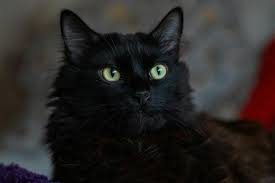
\includegraphics[width=0.9\textwidth]{images.jpg} \\
		\vspace{0.2cm}
		\footnotesize{\textit{Mi Gato Pickle}}

		% COLUMNA 2: LOS PASATIEMPOS
		\column{0.6\textwidth}
		\begin{block}{Actividades de Tiempo Libre}
			\begin{itemize}
				\item Jugar Minecraft
				\item Aprender más sobre Linux y su kernel
				\item Practicar Programación Competitiva
				\item Hacer judo, descenso y nadar
				\item Ver series de ciencia ficción
			\end{itemize}
		\end{block}

	\end{columns}
\end{frame}
\end{document}
